\section {Capacitor Parameters}
\subsection{Comments}
*In Section 3.1 you could mention what characteristics are important for that application.  And capacitors for switching power supplies are conspicuously absent.
*Do you want to get into capacitor parameters such as stability, temperature operating range, working voltage, peak or surge current, etc

\subsection{Practical Capacitor Uses}

Before getting into the individual capacitor parameters, I will explain some of the basic uses for capacitors. Each of the individual parameters will be important and have a direct effect on the uses described here. One should be careful to remember that any model consisting of the parameters listed in this section (and others) only describes an approximation of what is happening inside of a capacitor. Models and capacitor parameters will never be 100\% correct, but can be made with fairly high accuracy. As long as the designer understands the circumstances in which the models are accurate, he can use them to make a better circuit.

The most basic reason for wanting to use a capacitor is that it has the ability to store charge, which is close to the same thing as saying that it has the ability to store energy. It can store and release energy quickly to be able to react to the needs of the circuit.

\subsubsection{Power Supply Bypassing}

One of the most common uses for capacitors is to bypass a DC power supply. In the case of an Linear or DC-DC power supply, they are expecting a generally constant power supply. A portion of the noise (none DC voltage) on the line will be transferred to the output. Putting a capacitor from a power supply to ground acts as a local charge reservoir to smooth out noise on the line. See Figure \ref{bypassing}.

\begin{figure}
    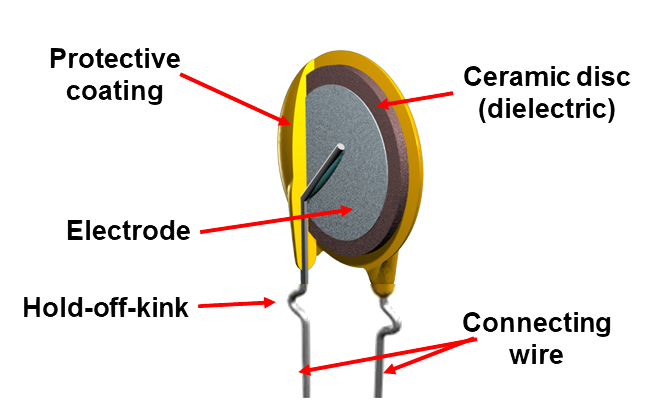
\includegraphics[keepaspectratio=true,scale=.5]{./figures/testImage.png}
    \centering
%    \cite{capSite_df_vs_temp}
    \caption{Bypassing Example}
    \label{bypassing}
\end{figure}

Bypass capacitors are also put close to the power pins on IC chips. Especially with digital chips, high frequency switching causes surges of current to be drawn from the line. If not for having bypass capacitors, this would cause dips in the power line at the switching frequency. This effect can cause logical glitches that are very difficult to debug.

\subsubsection{Analog Filtering}

Another use for capacitors is in analog filtering. Take for instance the low pass figure in Figure: \ref{lowPass}. The capacitor is used in this configuration to control which frequencies get passed to the rest of the circuitry. Low pass filters are needed in many application; a few of them being anti-aliasing, clock filtering, and integration.

\begin{figure}
    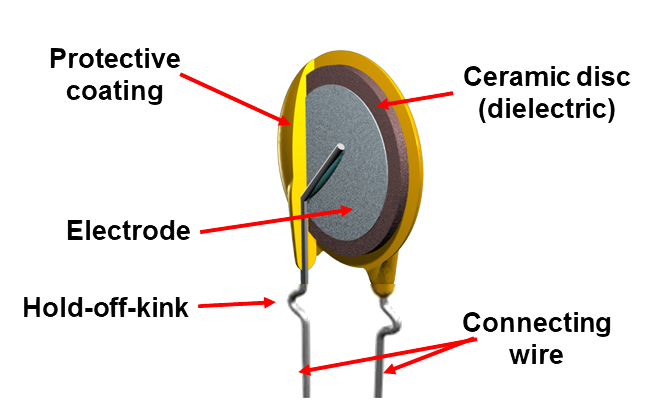
\includegraphics[keepaspectratio=true,scale=.5]{./figures/testImage.png}
    \centering
%    \cite{capSite_df_vs_temp}
    \caption{Low Pass Filter}
    \label{lowPass}
\end{figure}

\subsubsection{DC Blocking}

Designers often take advantage of capactors' characteristic of passing AC current while blocking DC current. As in Figure: \ref{dcBlock}, a capacitor can be used to block a DC offset before an amplifier. 

\begin{figure}
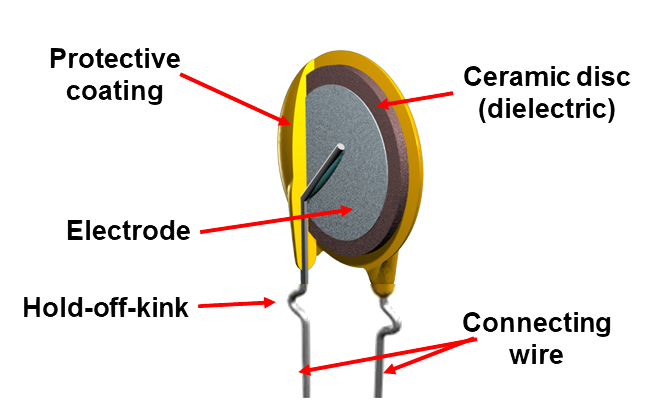
\includegraphics[keepaspectratio=true,scale=.5]{./figures/dcBlock.png}
\centering
%    \cite{capSite_df_vs_temp}
\caption{Using a capacitor in a DC blocking application}
\label{dcBlock}
\end{figure}



\subsubsection{Power Factor Correction}

The inductors in modern DC-DC switching supplies have required increased attention to the engineering phenomenon know as power factor. Any electrical load with an inductive component causes the supplied current phase to lag the voltage phase. This effect decreases the efficiency of the power distribution and also has the ability to cause stability issues. A capacacitor can be used as a simple, passive way to move the power factor back towards the ideal state (See Figure: \ref{powerFactor}). \cite{cui_powerFactor}
\begin{figure}[ht!]
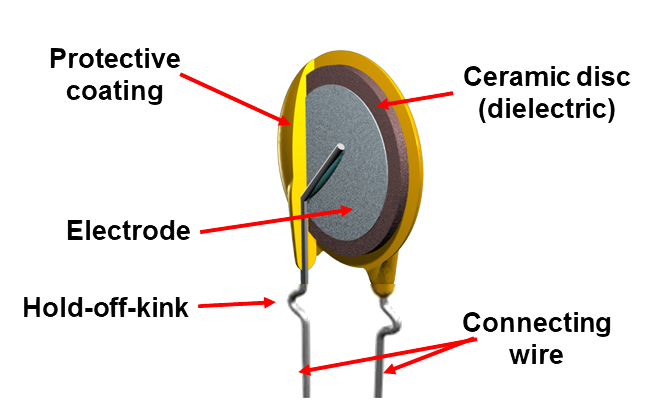
\includegraphics[keepaspectratio=true,scale=.5]{./figures/parameters/powerFactor.png}
\centering
\caption{Power Factor Correction Circuit}
\label{powerFactor}
\end{figure}



\subsubsection{Oscillators}
Capacitors are also used in oscillator circuits. -- Add resonator from HnH.

\subsection{Capacitance}

There is a distinct difference between a capacitor and capacitance. While a capacitor's main characteristic is capacitance, it cannot be modeled entirely as such in most practical applications. There are various inductive and resistive components to a capacitor that are important in various circumstances.

\begin{equation}
\label{cqv}
C=\frac{Q}{V}
\end{equation}

Capacitance is the ability to store electrical charge. Equation: \eqref{cqv} says that capacitance is stored charge that is spread throughout a volume. A device that can store a lot of charge in a small area has a large capacitance.The basic equation for a commercial capacitor is seen in Equation: \eqref{parPlateCap}.

\begin{equation}
\label{parPlateCap}
C = \frac{\epsilon _0 A}{d}
\end{equation}

When using a capacitor in a single-pole low-pass filter, the cutoff frequency can be determined by Equation: \eqref{lpfilter_eqn}. The circuit designer will choose a value for C and R in order to meet the cutoff frequency restraint.

\begin{equation}
\label{lpfilter_eqn}
f = \frac{1}{2\pi RC}
\end{equation}

Varying the capacitance used in the filter will move the cutoff frequency and consequently get a different response in the filter. The effect of this can be seen in Figure: \ref{lowPassFilt_fig}.

\begin{figure}
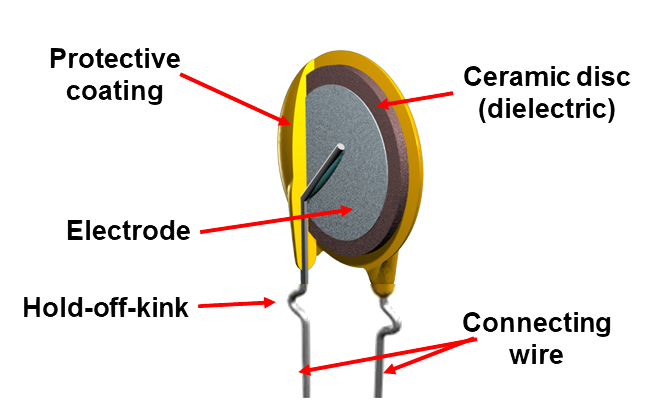
\includegraphics[keepaspectratio=true,scale=.5]{./figures/testImage.png}
\centering
%    \cite{capSite_df_vs_temp}
\caption{Changing Capacitance in a Low Pass Filter}
\label{lowPassFilt_fig}
\end{figure}

\subsection{Impedance}

The impedance of a capacitor is the "AC resistance" of the device. It determines the AC current that will flow when an ac voltage is applied to the capacitor via Ohm's law (Equation: \eqref{capOhmsEqn}). An ideal capacitor has no resistive elements and is purely capacitive. Therefore, its impedance can be described via Equation: \eqref{capImpEqu}. The two main things to notice are that the impedance is frequency dependent and it is purely imaginary (reactive).

\begin{equation}
\label{capOhmsEqn}
\vec{V} = \vec{I} \vec{Z}
\end{equation}

\begin{equation}
\label{capImpEqu}
\vec{Z} = \frac{1}{2\pi jfC}
\end{equation}

\begin{equation}
\label{capMagEqn}
Z = |\vec{Z}| = \frac{1}{2\pi fC}
\end{equation}

In most AC applications we look at the magnitude of the impedance. Real capacitors have a more complicated impedance, but with an ideal capacitor we can simplify the magnitude equation down to Equation \eqref{capMagEqn}

When capacitors are used in bypassing power supplies, the idea is to have a low impedance for common or expected noise frequencies. One may be tempted to choose a large valued capacitor to use for bypassing a wide range of frequencies. This turns out to backfire in practical situations, due to other parasitics in a real capacitor. For any capacitor, the impedance equation is more complicated, and the impedance value will begin to increase with frequency after some point. This will cause the designer to choose several different valued capacitors in parallel when bypassing a power supply or sensitive component. We will see later that the frequency plot of a capacitor will end up being more complicated than the simplified version seen in Figure: \ref{idealCapMagfig}.

\begin{figure}
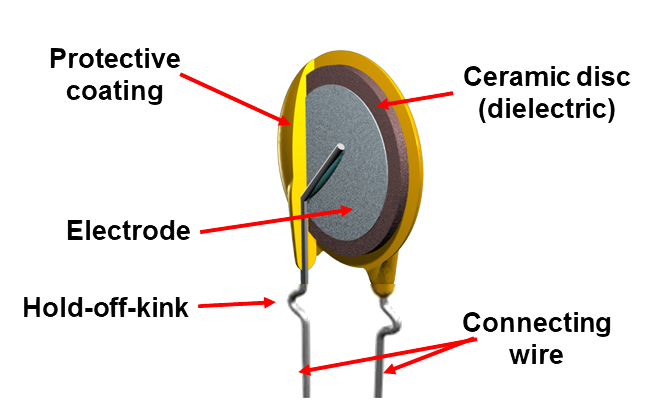
\includegraphics[keepaspectratio=true,scale=.5]{./figures/testImage.png}
\centering
%    \cite{capSite_df_vs_temp}
\caption{Ideal Capacitor Magnitude versus frequency}
\label{idealCapMagfig}
\end{figure}

\subsection{Phase}

The phase of a combination of resistive and reactive components can be written as in Equation: \eqref{capPhEqn}.

\begin{equation}
\label{capPhEqn}
\phi = tan^{-1}[\frac{X_c}{R_c}]
\end{equation}

For an ideal capacitor, having no resistance and only capacitance, the phase angle is only written as:

\begin{equation}
\label{capImpEqu2}
\phi = -i = -90^0
\end{equation}

The practical implication of this can be seen in the phase response of a low pass filter (Figure: \ref{lpFiltPhaseFig}). The capacitor introduces a phase lag relative to the input signal's frequency. If you would compare the input and output signals in time, the output's peak would lag behind the input's by the phase amount predicted in the phase response.

\begin{figure}
    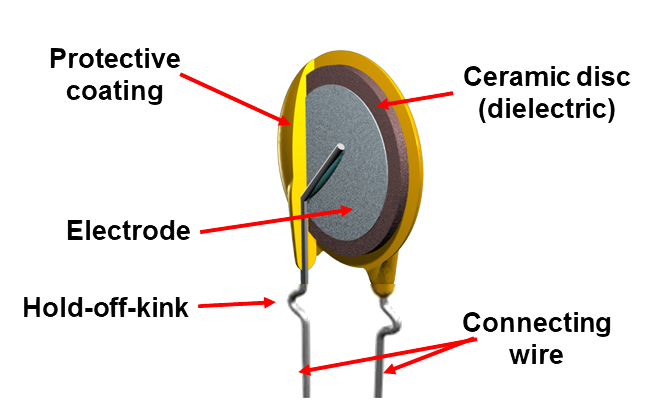
\includegraphics[keepaspectratio=true,scale=.5]{./figures/testImage.png}
    \centering
%    \cite{capSite_df_vs_temp}
    \caption{Low-Pass Filter Phase}
    \label{lpFiltPhaseFig}
\end{figure}

\subsection{ESL}

The Equivalent Series Inductance (ESL) of a capacitor is a lumped estimate of all of the inductive components of a capacitor. It is typically modeled as an inductor in series with the bulk capacitance (See Figure \ref{capESLModelFig}).

\begin{figure}
    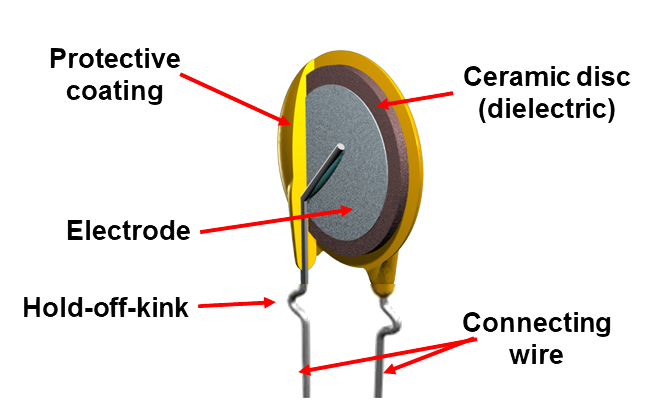
\includegraphics[keepaspectratio=true,scale=.5]{./figures/testImage.png}
    \centering
%    \cite{capSite_df_vs_temp}
    \caption{Capacitor ESL Model}
    \label{capESLModelFig}
\end{figure}

Adding ESL to the capacitive model creates a new impedance equation (Equation: \eqref{impESL}). Note that for L\textless \textless C, this equation simplifies to Equation: \eqref{capImpEqu} for low frequencies.

\begin{equation}
\label{impESL}
\vec{Z_c} = \frac{1-\omega ^2CL}{j\omega C}
%\cite{maxSwEff}
\end{equation}

\begin{equation}
\label{phaseESL}
\phi = Phase
%\cite{maxSwEff}
\end{equation}

Similarly, Equation: \eqref{phaseESL} shows that the phase of the capacitor is also affected at higher frequencies

\begin{figure}
    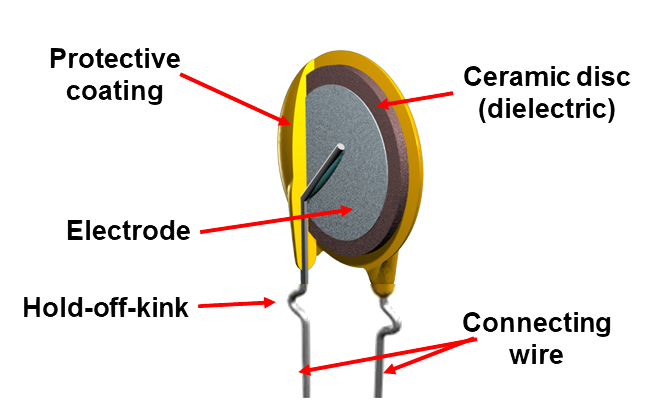
\includegraphics[keepaspectratio=true,scale=.5]{./figures/testImage.png}
    \centering
%    \cite{capSite_df_vs_temp}
    \caption{ESR+ESL Impedance-Phase Plot}
    \label{capESLPlot}
\end{figure}

Figure: \ref{capESLPlot} shows a graphical representation of a capacitor's magnitude and phase once ESL is considered. This plot shows that at a certain frequency, a capacitor's impedance will begin to increase with frequency. This means that a bypass capacitor will only be effective up to a certain frequency. Typically, the this frequency point and the capacitor's value have an inverse relationship. This is why you will see power supplies and sensitive chips being bypassed by a range of widely different valued capacitors. 

\subsection{ESR}
A real capacitor is more complicated than the ideal single capacitor model. One of the most used parameters is the Equivalent Series Resistance (ESR). ESR is the practical result of the fact that the materials used to create the capacitor have resistance. In simple cases, this can be approximated by a resistance in series with a capacitor (See figure: \ref{capESRModelFig}).

\begin{figure}
    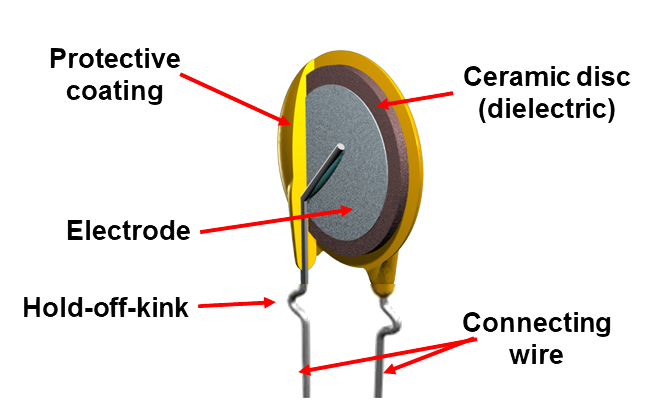
\includegraphics[keepaspectratio=true,scale=.5]{./figures/testImage.png}
    \centering
%    \cite{capSite_df_vs_temp}
    \caption{Capacitor ESR Model}
    \label{capESRModelFig}
\end{figure}

ESR becomes is important when thinking about DCDC switch mode power supplies. The converter's output voltage will have some ripple voltage on top of the DC output. This produces a ripple current through the capacitor. The capacitance element experiences no losses, but the ESR dissipates power according to Equation: \eqref{dcdcESReqn}

\begin{equation}
\label{dcdcESReqn}
P_{ESR} = I_{C,RMS}^2 * ESR
\cite{maxSwEff}
\end{equation}

\begin{equation}
\label{ImpCEslEsr}
\vec{Z_c} = ESR + j * (\omega L - \frac{1}{\omega C})
\cite{maxSwEff}
\end{equation}

Another important thing to note about ESR is that even though it is modeled as a resistance, it is not constant across all frequencies. It is a simplification of resistive and capacitive elements in a capacitor that are dominated by resistance.

\subsection{Resonance Frequency}

Once C, ESL, and ESR are included into the capacitor model, a parameter know as the self-resonant frequency becomes evident. Equation: \eqref{ImpCEslEsr} shows that when $Z_{ESL} == Z_C$, the capacitor is at its resonance point. At this frequency, the capacitor's impedance is determined solely by the ESR at that frequency. This frequency can be calculated by Equation: \eqref{fres}.

\begin{equation}
\label{fres}
f_r = \frac{1}{2\pi \sqrt{LC}}
\end{equation}

\subsection{Dissipation Factor}

Dissipation factor, otherwise known as the loss-tangent, is a measure of the energy stored to the energy dissipated per cycle. It is a measurement of the efficiency of the capacitor. The DF can be quantified through Equation: \eqref{dispFac}. 

\begin{equation}
\label{dispFac}
D = \frac{ESR}{Xc}
\end{equation}

\begin{figure}
    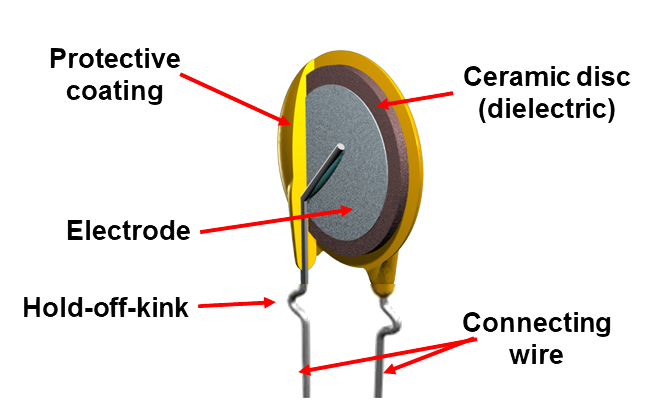
\includegraphics[keepaspectratio=true,scale=.5]{./figures/testImage.png}
    \centering
%    \cite{capSite_df_vs_temp}
    \caption{Dissipation Factor Plot}
    \label{dfPlot}
\end{figure}

The loss tangent can be seen in Figure: \ref{dfPlot}. The greater the angle, the more efficient the capacitor will be.

\subsection{Quality Factor}

\begin{equation}
\label{qual}
Q = \frac{1}{D}
\end{equation}

The Quality Factor, Q, of a capacitor is found by taking the reciprocal of the dissipation factor, Equation: \eqref{qual}. It is defined as the ratio of the energy stored to the energy dissipated per cycle.

\subsection{Insulation Resistance}

Every capacitor will have some DC leakage resistance associated with it. This measurement is attenuated by the insulation resistance of the capacitor. A high insulation resistance in a capacitor will increase its ability to store charge. This characteristic is especially important in sample and hold circuits.

\subsection{Dielectric Absorption}

Dielectric Absorption, DA, in a capacitor is a characteristic which describes the unit's ability to "regenerate" a charge after being shorted to ground for a brief time.

\begin{figure}
    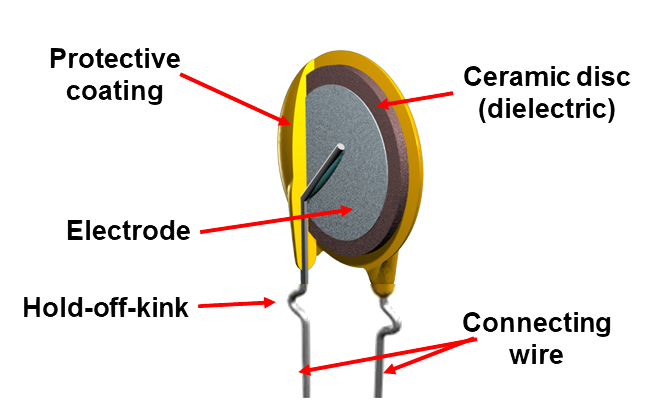
\includegraphics[keepaspectratio=true,scale=.5]{./figures/testImage.png}
    \centering
%    \cite{capSite_df_vs_temp}
    \caption{Dielectric Absorption}
    \label{daPlot}
\end{figure}

As seen in Figure: \ref{daPlot}, a capacitor can be modeled with multiple RC element, of a much greater time constant, in parallel with the bulk capacitance. When the main capacitor is shorted to ground, and then released, the other capacitors may not have released their energy. After several minutes, they can recharge the main capacitance to a significant portion of its original charge. This is why large valued electrolytic capacitors get shipped with a resistor across their terminals.

\subsection{Old}

This section will list and explain a large number of capacitor parameters. It will not deal with any analysis or measurement.

\begin {enumerate}
    \item Impedance
    \item Phase
    \item Capacitance
    \item Reactance
    \item Equivalent Series Resistance (ESR)
    \item Equivalent Series Inductance (ESI)
    \item Leakage current
    \item Dissipation factor
    \item Quality factor
    \item Dielectric absorption
    \item Loss Tangent
\end {enumerate}
